%%%%%%%%%%%%%%%%%%%%%%%%%%%%
%% Attention, ne pas faire de modifs directement dans ce fichier .tex
%% car il a �t� g�n�r� � partir d'un fichier .rbtex
%%%%%%%%%%%%%%%%%%%%%%%%%%%%


%\input{../annales.sty} % le dessin est dans PS/, annales.sty dans le
                       % rep parent
%\usepackage{tikz} % la base
%\usetikzlibrary{calc,through,backgrounds}

% Si la compilation de ce fichier �choue avec l'erreur
%	! Package xkeyval Error: `babel' undefined in families `MT',
% commentez la ligne suivante.
%\usepackage[babel=true,kerning=true]{microtype} % pour resoudre un
                                % probleme de compatibilite entre
                                % [francais]{babel} et TikZ/PGF.
%\usepackage{aeguill}   % Pour forcer une police vectorielle
%\pagestyle{empty} % On veut le dessin seul
%\begin{document}

\newcommand{\POLAIREUN}[1]{\begin{tikzpicture}

\pgfmathsetmacro{\t}{#1}
\pgfmathsetmacro{\R}{2.4 + 0.6*cos(\t)}
\pgfmathsetmacro{\UNIT}{0.7}
\pgfmathsetmacro{\THETA}{45 - 20*sin(\t+45)}

%% Les valeurs utiles



\clip (-1.2,-0.7) rectangle (3.60000,3.60000) ;


\draw (0,0) circle (\R) ;

\coordinate (M) at ({\R*cos(\THETA)},{\R*sin(\THETA)}) ;

\draw [ultra thick, ->] (0,0) -- (M) node [pos=0.5,above left=-2pt] {$r$};

\filldraw [black] (M) circle(2pt) node [below=-4pt] {\quad\ \ $M$};
\filldraw [black] (0,0) circle(2pt) node [below left=-2pt] {$O$};

%% Les axes

\draw [->] (0,0) -- (3.3,0) node [above] {$x$} ;
\draw [->] (0,0) -- (0,3.3) node [left] {$y$} ;

%% Les projections

\draw [dashed] ({\R*cos(\THETA)},0) node [below] {$r\cos\theta\quad$}
	-- (M) --  (0,{\R*sin(\THETA)}) node [left]  {$r\sin\theta$} ;

%% Les vecteurs

\draw [->,ultra thick] (0,0) -- (0.7,0) node [below] {$\vex$} ;
\draw [->,ultra thick] (0,0) -- (0,0.7) node [left] {$\vey$} ;

\draw [->,ultra thick,shift=(M),rotate=\THETA] (0,0) -- (1,0) node [above] {$\ver$} ;
\draw [->,ultra thick,shift=(M),rotate=\THETA] (0,0) -- (0,1) node [above] {$\vetheta$} ;

%% L'arc de cercle

%\draw [thick,->] (1.20000,0.0) -- (1.19980,0.02166) -- (1.19922,0.04332) -- (1.19824,0.06497) -- (1.19687,0.08659) -- (1.19511,0.10818) -- (1.19297,0.12974) -- (1.19043,0.15126) -- (1.18750,0.17273) -- (1.18419,0.19414) -- (1.18049,0.21549) -- (1.17641,0.23676) -- (1.17194,0.25796) -- (1.16710,0.27908) -- (1.16187,0.30011) -- (1.15626,0.32103) -- (1.15028,0.34186) -- (1.14392,0.36257) -- (1.13718,0.38316) -- (1.13008,0.40363) -- (1.12261,0.42397) -- (1.11477,0.44417) -- (1.10657,0.46422) -- (1.09801,0.48412) -- (1.08909,0.50387) -- (1.07982,0.52345) -- (1.07019,0.54286) -- (1.06021,0.56209) -- (1.04989,0.58114) -- (1.03923,0.60000) ;
\draw [thick,->] (1,0) arc (0:\THETA:1) ;

\draw ({\THETA/2}:1) node [right] {$\theta$};



%\draw [dashed] (M) circle (0.28) ;

%\draw [dotted,shift=(M)] (0,0.28000) 
%	-- (4,1.1) ;

\end{tikzpicture}}

\newcommand{\POLAIREDEUX}[1]{%
\begin{tikzpicture}[scale=3]

\sisetup{round-mode=places,round-precision=1}

\pgfmathsetmacro{\t}{#1}
\pgfmathsetmacro{\R}{2.4 + 0.6*cos(\t)}
\pgfmathsetmacro{\UNIT}{0.7}
\pgfmathsetmacro{\THETA}{45 - 20*sin(\t+45)}
\pgfmathsetmacro{\iTHETA}{int(\THETA)}
\pgfmathsetmacro{\dR}{0.4}
\pgfmathsetmacro{\dTHETA}{10}


  \coordinate (O)  at (0,0) ;
  \coordinate (M)  at (\THETA:\R) ;
  \coordinate (Mr) at (\THETA:{\R+\dR}) ;
  \coordinate (Mt) at ({\THETA+\dTHETA}:\R) ;
  \coordinate (B)  at ({\THETA+\dTHETA}:{\R+\dR}) ;
  \coordinate (I)   at (barycentric cs:Mt=0.5,M=0.5,Mr=0.5,B=0.5);
  \coordinate (J)   at (barycentric cs:O=0.1,M=0.9);
  \coordinate (K)   at (barycentric cs:O=0.1,Mt=0.9);
  \coordinate (L)   at (barycentric cs:J=0.5,K=0.5);

  \draw (I) ++ (0,0.55) node {{$r=\num{\R}$, $\theta=\iTHETA$\textdegree}} ;
  \clip [draw] (I) circle (0.7);
%  \draw [dashed] (I) circle (0.7) ;
 
  \filldraw [black] (M) circle (0.5pt) node [below] {$M$};
%  \filldraw [black] (0,0) circle (0.5pt) ;
%  \filldraw [black] (Mt) circle (0.5pt) node {$M_\theta$} ;
%  \filldraw [black] (Mr) circle (0.5pt) node {$M_r$} ;
%  \filldraw [black] (B) circle (0.5pt) node {$B$} ;
  \draw (0,0) -- (M) ;
  \draw [dashed] (Mr) -- (\THETA:{2*\R}) ;
  \draw [dashed] (B)  -- ({\THETA+\dTHETA}:{2*\R}) ;
  
  \draw (0,0) -- (Mt);
  
  \filldraw [fill=gray] (Mt) -- (B) 
    arc ({\THETA+\dTHETA}:{\THETA}:{\R+\dR})
    %(2.60455,2.18548) -- (2.64644,2.13456) -- (2.68734,2.08284) -- (2.72722,2.03034) -- (2.76608,1.97707) -- (2.80390,1.92306) -- (2.84066,1.86833) -- (2.87635,1.81290) -- (2.91097,1.75678) -- (2.94449,1.70000)
  	-- (M)  
    arc (\THETA:{\THETA+\dTHETA}:\R)
    %(2.59808,1.50000) -- (2.56850,1.55010) -- (2.53796,1.59961) -- (2.50646,1.64853) -- (2.47403,1.69682) -- (2.44066,1.74448) -- (2.40637,1.79148) -- (2.37118,1.83780) -- (2.33509,1.88344) -- (2.29813,1.92836)
    ;
  
  \draw [ultra thick,->] (M) -- (Mr) node [above=5pt] {$\quad\ \dd r\ver$}; 
  \draw [ultra thick,->] (M) arc (\THETA:{\THETA+\dTHETA}:\R) 
  		node [left=-2pt] {$r\dd\theta\vetheta$};

\pgfmathsetmacro{\nbPOINTS}{10}

  \draw [ultra thick,->] (M) 
     \foreach \x in {1,...,\nbPOINTS} {
       -- ({\THETA + \x*\dTHETA/\nbPOINTS}:{\R+\x*\dR/\nbPOINTS})
     }
  		node [left] {$\dd\vect{OM}$};

  \draw [<->] (J) arc (\THETA:{\THETA+\dTHETA}:{0.9*\R}) ;
  \draw (L) node [above right=-3pt] {$\dd\theta$} ;

\end{tikzpicture}}

\def\CIRCULAIRE{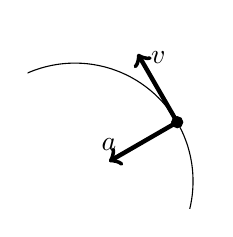
\begin{tikzpicture}[scale=0.5]

\clip (-1.2,-0.7) rectangle (3.30000,3.90000) ;

\coordinate (M) at (2.59808,1.50000) ;
\coordinate (O) at (0,0);

\draw (O) circle (3) ;

\filldraw [fill=black] (M) circle (4pt) ;

\draw [ultra thick,->,shift=(M)] (0,0) -- (-1.00000,1.73205) node [pos=0.95,right] {$\vect{v}$};

\draw [ultra thick,->] (M) -- (0.86603,0.50000) node [pos=1,above] {$\vect{a}$};

\end{tikzpicture}}

\def\ACCELERE{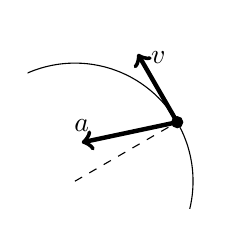
\begin{tikzpicture}[scale=0.5]

\clip (-1.2,-0.7) rectangle (3.30000,3.90000) ;

\coordinate (M) at (2.59808,1.50000) ;
\coordinate (O) at (0,0);

\draw (O) circle (3) ;

\filldraw [fill=black] (M) circle (4pt) ;

\draw [ultra thick,->,shift=(M)] (0,0) -- (-1.00000,1.73205) node [pos=0.95,right] {$\vect{v}$};

\draw [ultra thick,->] (M) -- (0.17365,0.98481) node [pos=1,above] {$\vect{a}$};
\draw [dashed] (O) -- (M) ;

\end{tikzpicture}}

\def\RALENTI{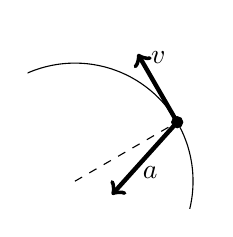
\begin{tikzpicture}[scale=0.5]

\clip (-1.2,-0.7) rectangle (3.30000,3.90000) ;

\coordinate (M) at (2.59808,1.50000) ;
\coordinate (O) at (0,0);

\draw (O) circle (3) ;

\filldraw [fill=black] (M) circle (4pt) ;

\draw [ultra thick,->,shift=(M)] (0,0) -- (-1.00000,1.73205) node [pos=0.95,right] {$\vect{v}$};

\draw [ultra thick,->] (M) -- (0.93969,-0.34202) node [pos=0.7,right] {$\vect{a}$};
\draw [dashed] (O) -- (M) ;

\end{tikzpicture}}
